
\section{Case Definitions}

This paper proposes siting a borehole
 repository at a shut down nuclear power plant such as one similar to the 
 Clinton Power Plant in Illinois. This proposed case is then compared to a 
 reference case at Yucca Mountain. Finally, a third case including repsitories 
 at both sites is considered.  The details of these three scenarios are described in this section.

 For comparison's sake, all three cases include a borehole-type repository concept, and are compared 
 primarily with respect to the benefits of the three siting strategies.
The borehole design follows the Sandia Report Reference Design and Operations 
for Deep Borehole Radioactive Waste \cite{arnold_reference_2011}. Selection of 
an alternative borehole concept could impact the details of the repacking needs 
and facility design, but will not significantly impact the siting comparison 
here.
 
\subsection{Case I: Reference Case} 
The reference case, upon which the proposed case seeks to improve, is to build 
a standalone 70,000 \gls{MTHM} borehole repository at the Yucca Mountain site.

The reference case is presented in order to demonstrate the cost savings and efficiencies 
that arise from the proposed case. The base case mimics the Yucca Mountain Project
but is a borehole-type repository. Costs include new licensing and processing facilityfor repacking the spent fuel assemblies.

\subsection{Case II: Shut Down Plant Case}

The imminent shutdown of the Clinton Nuclear Power Station has recently been 
averted by an act of the state legislature. In this sense, Clinton is 
representative of a class of at-risk nuclear 
reactors in the midwest and eastern United States. A borehole repository 
sited at the Clinton Nuclear Power station site is therefore hypothetically 
considered here to represent integrated repository siting at a reactor facility 
faced with potential shutdown.

The Clinton Nuclear Power Station is owned by the Exelon Corporation. It has a 
licensed land area of approximately $58km^2$ and a $20km^2$ cooling heat sink, 
the Clinton Lake. Of the licensed land area, only $.6km^2$ is used for the facility.  
\cite{nrc_chapter_2007}.  This leaves enough room left for a 70,000 \gls{MTHM} 
borehole repository without additional land purchase from the public.

\subsection{Case III: Combined Case}
Finally, given that one 70,000 MTHM repository is already insufficient for 
domestic \gls{SNF} needs \cite{doe_report_2008}, a final case can be proposed, 
a dual-repository scenario. In this scenario, both the Yucca Mountain 
repository and the near-Clinton borehole repository are sited and someday 
become operational. The proposal that a pair of repositories, east and west, is 
not new. Indeed, it was originally envisioned before the Yucca Mountain site 
selection was made.

In this scheme, eastern reactors send their spent fuel to the eastern 
repository site while wastern reactors send theirs to the western site. Thus, 
the less-nuclear western region will not bear the burden of hosting a 
repository for the eastern region, which has a higher percent of nuclear 
energy. 

For this scenario, spent fuel west of the 92 west meridian is considered west, 
which will send its \gls{SNF} to Yucca Mountain. Conversely, spent fuel east of the 92 west
meridian is considered east, which will send its \gls{SNF} to the proposed Clinton 
power plant. The 92 west meridian is chosen because it is the meridian just west of
Illinois state borders, so that no Illinois power plants have to transport their
spent fuel to Yucca Mountain. %no division.



\section{Evaluation Metrics}

To quantify the benefits of this repository design, a set of metrics are 
proposed:

\begin{itemize}
        \item Transportation Burden $[MTHM \cdot km]$: A site is preferred by 
                most stakeholders if it can minimize the distance \gls{SNF} 
                must travel.
        \item Job Creation $[\#]$: A repository concept is preferred by 
                government and community stakeholders if it is a source of 
                jobs. 
        \item Workforce Utilization $[\$]$: A repository site is preferred by 
                many stakeholders if it utilizes an already skilled local 
                workforce. 
        \item Expediency $[y]$: Many stakeholders will benefit if the removal 
                of dry casks from current storage pads is expedited.
        \item Consent Basis $[\frac{MW}{\mbox{person}}]$: If there is a basis for a consent-based 
                siting process to succeed, many stakeholders benefit.
        \item Site Access $[-]$: Rail access to the site is essential for 
                beginning operations.
        \item Site Appropriateness $[-]$: A site must be geologically 
                appropriate, of sufficient area, etc.
\end{itemize}

To model the impact of these measures on the incentives of each stakeholder, 
the list of stakeholders considered follows in Table \ref{tab:stakeholders} 
alongside the weights indicating the magnitude of the importance of the incentive.
 
\begin{table}[h]

\centering
\caption {Metrics and Weight for Each Stakeholder}
\scalebox{0.65}{
	\begin{tabular}{|l|l|l|l|l|}
	\hline
	 & Federal & State & Local & Utility  \\ \hline
	Job Creation &   & 1 & 3 & 1    \\ \hline
	Consenting Locals & 3 & 2 & 3 & \\ \hline
	Transport & 2 & 1 & 2 & \\ \hline
	No Need for additional land purchase & 3 & 2 & 3 &  \\ \hline
	Cease of Dry Storage Campaigns & 3 & & & 3  \\ \hline
	Net Cost & 3 & & & 3  \\ \hline
	No New Above-Ground Facility Construction & 3 & & & 3 \\ \hline
	
	\end{tabular}}
\end{table}

These metrics and their definitions draw upon previous 
\cite{freeze_siting_2015,waleed_regional_2015} as well as original work.  In the 
following sections, the metrics are defined in more detail. In 
the final section, they are applied to comparatively evaluate each 
case.

\subsection{Transportation Burden}
 In order to minimize transport cost, a central location is preferred. To 
 capture this, a metric 
 for representing the distance a mass of spent fuel must be transported, the 
 transport burden, is introduced. This transportation burden is the product 
 of the \gls{SNF} mass and the distance it has to travel from its current 
 storage location to the proposed repository. This results in a 
 metric in units of $MTHM\cdot km$. 

 To arrive at the transportation burden for each case, a distance analysis was 
 completed using the Haversine formula \cite{shumaker_astronomical_1984}. 
 First, the coordinates of each power plant were obtained by scraping public 
 data \cite{wikipedia}.  The distance between each storage site (i.e. reactors 
 and \gls{ISFSI}) was then calculated by using the Haversine formula on the 
 geographical coordinates of the recieving and sending sites (1 and 2). 

 \begin{align} 
         \Phi_1,\Phi_2&= \mbox{latitude, radians}\\
         \lambda_1,\lambda_2 &= \mbox{longitude, radians}\\
         \Delta\lambda &= \left|\lambda_1 - \lambda_2\right|\\
         \Delta\Phi &= \left|\Phi_1 - \Phi_2\right|\\
         a&=\sin^2(\Delta\Phi)+\cos(\Phi_1)\cos(\Phi_2)\sin^2{\left(\frac{\Delta\lambda}{2}\right)}\\
         c &= 2arctan2(\sqrt{a},\sqrt{1-a})\\
         d &=  (6,371km)c
 \end{align}


Finally, this distance is multiplied by the \gls{MTHM} that needs to be 
transported from each sending site.

\begin{align}
        b_i &= m_id\\
        B &= \sum_i^N b_i\\
        \intertext{where}
        b_i &= \mbox{spent fuel transport burden from facility i}\\
        m_i &= \mbox{mass at facility i}\\
        B &= \mbox{total spent fuel transport burden}\\
        N &= \mbox{total number of facilities with spent fuel on site.}
\end{align}

This analysis used GC-859 spent fuel inventory data availalbe from \gls{EIA} 
through private communication \cite{domenico_GC-859_2016} as well as \gls{CURIE}, a web interface to 
the \gls{ORNL} universal database\cite{ornl_centralized_2016}.
From the list of 74 reactors, several candidates which minimize $B [MTHM\cdot 
km]$, spent fuel transportation burden, are listed below:
    
\begin{table}[h]
\centering

        \caption { Reactors with relatively small spent fuel transportation burden $ [MTHM\cdot km]$.}
    \scalebox{0.86}{
	\begin{tabular}{l|l|l|l}
	\hline
	Reactor & State & $MTHM*km$ & License Area [$km^2$]  \\ \hline
	Clinton & Illinois &  \textbf{77,352,339} & \textbf{57.87}   \\ \hline
	Peach Bottom & Pennsylvania & 85,563,135 & 2.509   \\ \hline
	Indian Point &   New York & 84,097,374 & .967   \\ \hline
	Dresden & Illinois &  \textbf{77,663,969} & 3.856   \\ \hline
	
	\end{tabular}}
\end {table}


However, this partitioning assigns the Yucca Mountain site approximately 
$14,000 [MTHM]$ of \gls{SNF}, much less than its proposed capacity of 70,000 MTHM. On the other hand, 
the Clinton repository \gls{SNF} burden woud be reduced to 61,777 MTHM. The transportation burden is 
$53,945,200 [MTHM\cdot km]$  
for Yucca Mountain, and $17,940,959 MTHM\cdot km$ for the Clinton repository. This 
adds up to a sum of 71,886,160 $MTHM\cdot km$, which is about 7\% less than that
of Clinton repository alone. This does not provide a comparable advantage. Other
reactor sites were tested in the transportation burden analysis but also failed
to provide a substantial advantage. Also, the selection of different reactors
were limited by the geological constraints, which is shown in figure 2.  

If the power total MTHM value were to be equal, a line is drawn at the 84 west
meridian, which yields $39,942 MTHM$ for the east repository, and $36,649 MTHM$ for
the Yucca Mountain repository. One of the original candidates, the Peach Bottom
reactor in Pennsylvania is then chosen for its central location in the east area.
However, this analysis yields a $MTHM\cdot km$ value of $92,575,081 MTHM\cdot km$,
which is substantially larger than that of having one repository in Clinton. 
Also, the Peach Bottom reactor site has little licensed land, which will require
additional land purchase for the repository. 

%transition??

The Clinton Power Plant is chosen as the site for the proposed case due to its
        low $MTHM\cdot km$ value and substantially large license 
        area\cite{nrc_chapter_2007}.
 Considering that only
 $30km^2$ is required for all the total \gls{SNF} amount, the licensed area at Clinton
  power plant allows more than  enough space to site a borehole repository, which
   avoids possible conflicts with the community from purchasing and utilizing more
    land. 
  
  The proposed case requires a great amount of cooperation from the utility that owns
  the Clinton power plant, Exelon Corporation. 
  Exelon has an incentive to cooperate,
  since it will earn profit throughout the construction and operation of the 
  repository at its power plant, as well as to utilize the currently idle land mass
  in a lucrative manner. Also, Exelon would be able to save on decommissioning of
  Clinton by selling the property as well as the infrastructure to the government 
  for the repository instead of decommissioning it.  
  
  %Currently, Exelon has no 
  %incentive to cooperate, for they do not pay for storage of spent fuel, due to 
  %the 2004 settlement with the Department of Justice. Also, Exelon currently owes
  %approximately a billion dollars to the \gls{NWF},
  %(gaining interest at U.S. Treasury bond rate) when a repository is completed
  %\cite{Ewing_2009}.
  
  
  The figure below demonstrates the geologic fitness of the proposed site, where 
  a crystalline basement lies at a depth of less than 2,000 meters.



\begin{figure}[!h] 
  \centering
  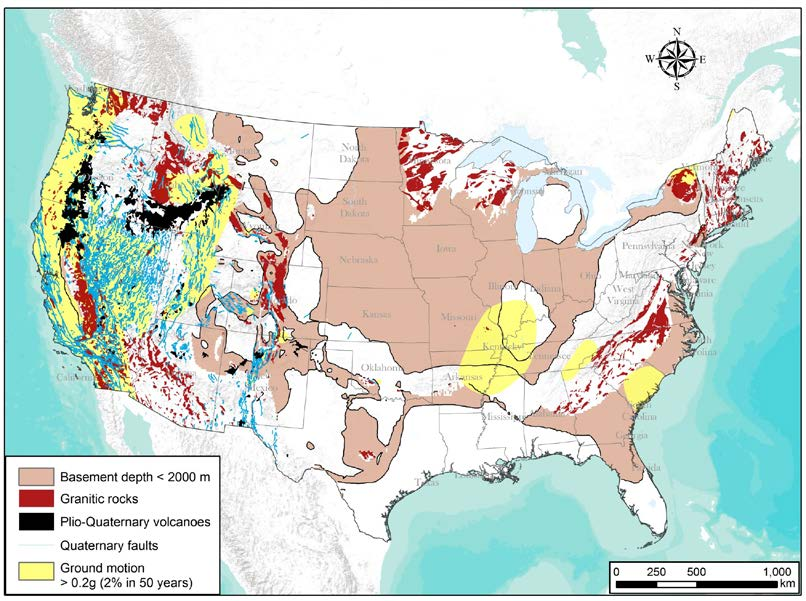
\includegraphics[width=0.8\columnwidth]{cbrock.png}	
        \caption{From \cite{perry_gis_2015}, a map of areas in the US with 
        crystalline basement rock at less than 2000 meters depth. Tectonic 
        activity impacting siting considerations are also mapped:  Quaternary 
        faulting, volcanism, and seismic hazard (yellow shading = 2\% 
        probability of exceeding 0.2 g in 50 years).}
  \label{fig:cbrock}
\end{figure}

  
  \iffalse

  %ommitted due to lack of space
\begin{figure}[!h] 
  \centering
  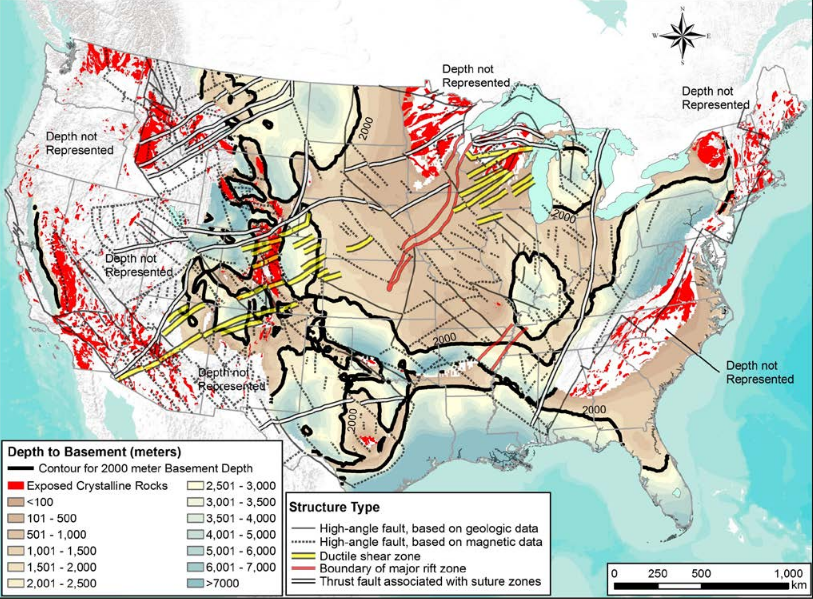
\includegraphics[width=0.8\columnwidth]{Crystalline-Thickness}	
  \caption{Depth of Crystalline Rock
  \cite{perry_gis_2015}.}
  \label{fig:Depth}
\end{figure}

 \fi
  
  
  Also, from the Decatur Carbon Sequestration Project, there is ample data
  on the stratigraphy of the Decatur region, which is less than 50 miles south
  of the Clinton power plant.
 
  
  
  
\begin{figure}[!h] 
  \centering
  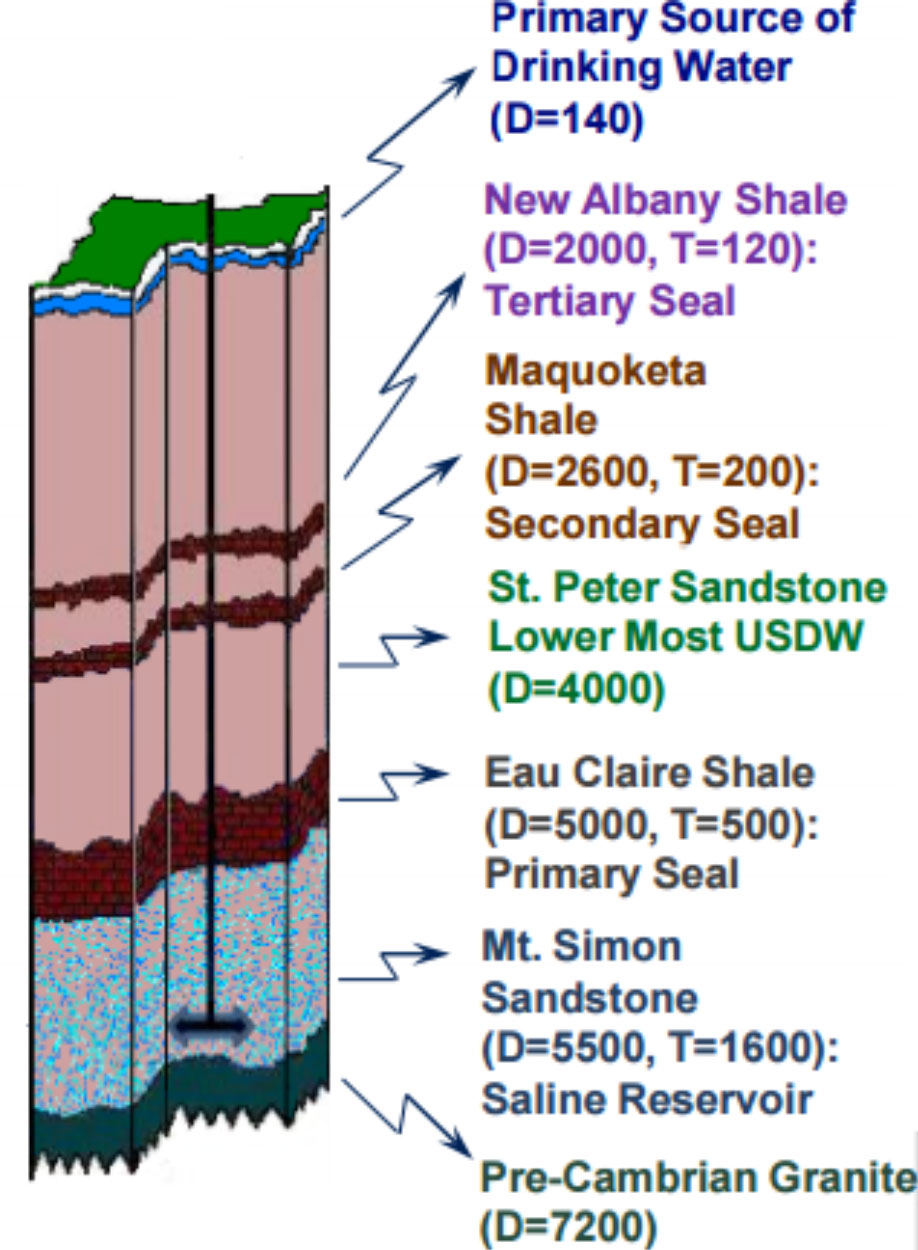
\includegraphics[width=0.8\columnwidth]{Stratigraphy-Decatur}	
  \caption{Stratigraphy of the Decatur Region
  \cite{mcdonald_illinois_2012}.}
  \label{fig:Stratigraphy}
\end{figure}
  

\subsection{Workforce Utilization}

%look at singer slides
% district 51 gets continuous property tax and benefits from the site (singer slides)
%%something about the state?
%utility can offer jobs preferrably to the workers being laid off to the repo
%really drive home the consent-based approach (sweden)


Building a spent nuclear fuel repository is no easy task. It is a task that requires
numerous experts and labourers. Also, operating and maintaining a nuclear power plant
requires numerous experts and labourers. In case of the proposed case, the Clinton
 Power Station has approximately 700 employees living in nearby counties with an
additional several hundred contractors during fuel 
outages\cite{exelon_clinton_2016}.
The existing skilled workers and local talent for maintenance, transport and catering
services can be utilized without bringing a whole new group of workers to the 
area \cite{iaea_managing_2008}. Also, the shutdown of Clinton Power Plant would cause a dramatic
loss of jobs in the community. 


%why is there such a huge difference between Riddel and Loomis?


The void created by the shutdown of the Clinton plant can be, though not
completely, filled by the new construction of a borehole repository. The construction
will prioritize local hires as an incentive to ease local opposition on repository
 siting. Employment during the operation of Yucca Mountain was estimated to range from
 2,000 to 5,000 jobs, \cite{riddel_economic_2003} which means that the borehole repository
 would at least require half of the workforce for the same capacity. 

Additionally, an estimate by the Illinois State University on fracking the New Albany
Shale in southern Illinois estimated that such a project can create 1,000-47,000 jobs
\cite{loomis_potential_2012}. Translating the workforce to central Illinois and the borehole
project should create somewhere in the low and medium estimate, which is about 10,000
jobs.   
%on top of everything we talked about,

%facilities involved,
%transportation of human/material resources and talent
%

The proposed case has a larger advantage over the base case in the sense that there
are already existing facility in regards to spent fuel handling and worker lodging 
and catering services. 
It is assumed, for the sake of argument, half of the construction cost of the
repacking facility in the base case is used to expand the existing facility in the
proposed case. 


\subsection{Consent Basis}
International \gls{SNF} siting experiences have shown that a consent-
based approach to siting a repository is crucial to success
\cite{ayers_blue_2012,doe_designing_2016,jenkins-smith_public_2013,freeze_siting_2015}. 
Further more, the Swedish precedent \cite{olsson_experiences_2013} shows that 
municipalities near nuclear facilities
are more likely to volunteer to site a repository in their community.

Since populations local to operating reactor sites are more likely to be 
favorable toward nuclear power, and the proposed integrated siting 
is in an already-nuclear community by design, this siting strategy inherently 
maximizes the local consent basis.

The source of this favorable attitude varies by site. 
the local community is the beneficiary of various economic benefits
including job creation and the substantial property taxes paid by the utility 
toward regional governmental budgets.   In the case of the Clinton Power Plant, 
Exelon pays \$15 million in property taxes each year, which amounts to about 
\$923 per resident in the host Dewitt county \cite{brady-lunny_dewitt_2016}. The plant
also provides a total payroll of more than \$50 million to its workers.
The eventual shutdown of the plant would have caused a dramatic loss of the economic inflow.
It is also speculated that 13,300 jobs would be lost in Illinois after five years 
of plant shutdown \cite{reid_study:_2014}.  

A similar phenomenon might be expected at the state level as well, since 
Illinois generates more nuclear energy than any other U.S.  state with a net 
capacity of 11,441 megawatts in 2010 \cite{eia_state_2012}. Nevada, on the other 
hand, hosts zero nuclear power plants. Thus, it can only be natural for Nevada 
to consider a national repository as an unjust burden, despite economic 
benefits.  

The consent basis, driven by proximity to an operating nuclear plant and 
corresponding greater likelihood to be favorable toward hosting an \gls{SNF} 
repository, should be quantifiable by a measure of the benefit experienced by 
the community.  For simplicity, we quantify the proximity to nuclear energy at 
the state level  based on power consumed. The corresponding state and regional 
metrics (expressed in MW of nuclear power per capita) are listed below. This 
analysis uses nuclear power generation capacity and population data from the 
U.S. \gls{EIA} \cite{eia_state_2012} and the U.S. Census \cite{census}.  

\begin{table}[h]
	
	\centering
	\caption {\gls{NMWPC} values for different states}

	\scalebox{0.60}{
		\begin{tabular}{|c|c|c|c|c|}
			\hline
			State & Net Nuclear Capacity (MW) & Census Population & \gls{NMWPC} ($10^{-3}$) \\ \hline
			South Carolina & 6,486 & 4,625,401 & 1.4 \\ \hline
			Alabama & 5,043 & 4,780,127 & 1.05 \\ \hline
			Vermont & 620 & 625,745 & .99 \\ \hline
			Illinois & 11,441 & 12,831,549 & .89 \\ \hline
			Nevada & 0 & 2,705,000 & 0 \\ \hline
			Average Nuclear States & 101,167 & 265,386,569 & .38 \\ \hline
			Average National & 101,167 & 309,300,000 & .33 \\ \hline
			
		\end{tabular}}
	\end{table}
	
	%centerit
	
The state of Illinois has the highest generating capacity, and is fifth in the \gls{NMWPC}
 value, while Nevada has zero generating capacity with zero MW per capita value. 
Illinois' \gls{NMWPC} value is also well above the national average. Judging from the
table, it is no surprise that the state of Nevada rejected the idea of having a national
spent fuel repository in its land. On the other hand, Illinois is more familiar with 
nuclear and also somewhat reliant on nuclear, which can lead to a consent-based process
in a state-level. 

	 

\subsection{Site Access}

%%% NWPA allows only "Transshipment of spent nuclear fuel to another civilian 
%%% reactor within the same utility system" [Title I, Subtitle B, Sec. 134(a)]

%further discussion on the railline and maybe numerically express each repository's
%proximity to closest transportation method?

%Federal: less transport, the better
%history of transport of SNF in-state?

Site access necessary to transport radioactive material to the repository site 
poses one of the greatest logistical challenges in siting a repository. 

In the case of Yucca Mountain, 
the opposition from the state of Nevada to the proposed Caliente rail corridor 
blocked construction of the rail line and indefinitely postponed
acceptance of \gls{SNF} at Yucca Mountain \cite{halstead_yucca_2011}.

Operating reactors, conversely, are much more likely to be located along rail 
lines. In the case of the Clinton nuclear power plant, 
the Canadian National rail line \cite{waleed_regional_2015} has a station in 
Clinton and dedicated tracks leading into the reactor facility, as shown in 
Figure \ref{fig:cnmap}.

An already existing railway can avoid costs and delays related to building a 
new infrastructure.

\begin{figure}[!h] 
  \centering
  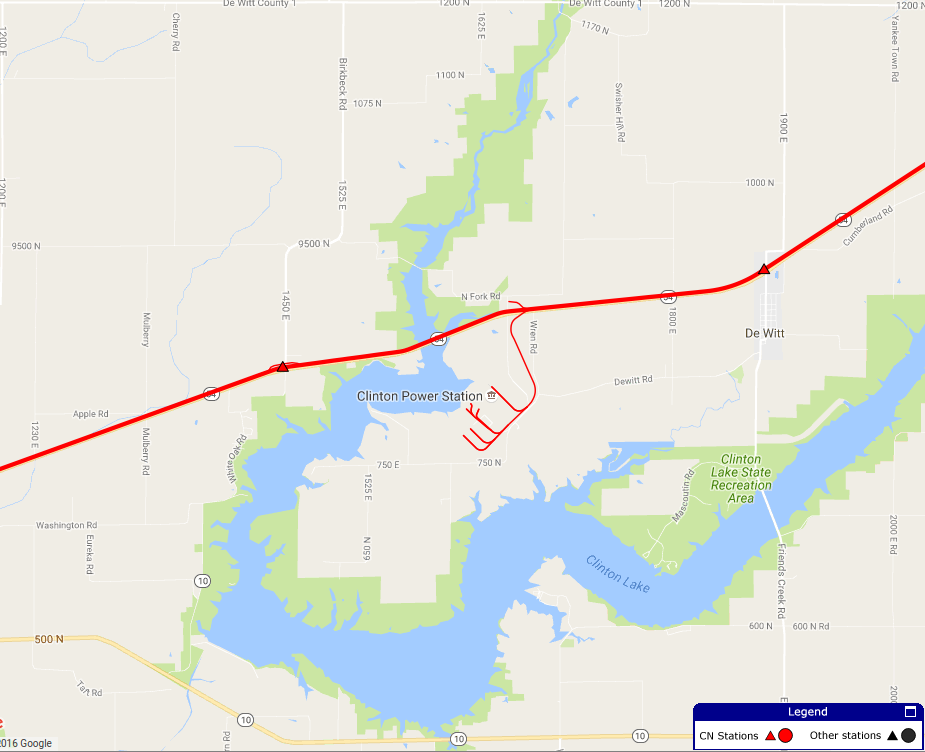
\includegraphics[width=0.8\columnwidth]{cnmap.png}	
        \caption{From \cite{canadian_national_railway_company_canadian_2016}, a map of Clinton Power Station in Clinton,IL
        with the Canadian National rail passing through.}
  \label{fig:cnmap}
\end{figure}

The proposed site's proximity to other power plants means that the transport
routes trespass less states and communities, which lessens conflict.

The capacity of the state to handle nuclear materials is also important.
The state of Illinois established a Division of Nuclear Safety in its \gls{IEMA}
which connects the state police and the Illinois Commerce Commission (ICC) to
 successfully transport 480 shipments of spent nuclear fuel since 1983
 \cite{iema_illinois_2005}. If a repository is built and operational, the already existing,
 experienced state organization will be able to handle the transportation logistics
 and security.  

Conversely, the base case has a $km*MTHM$ value of $209,575,157 km*MTHM$, 
which is approximately 2.7 times more than that of the proposed case. Also, the 
transportation route to Yucca Mountain is identified to traverse 955 counties
with about 177 million persons, which is about 56\% of the US total
 \cite{halstead_yucca_2011}. The trespass is a sensitive topic to some states, and may
 demand reroutes that cause unexpected cost increases in transportation. Also,
 new railways would need to be constructed in order to ship the spent fuel inventories
 by rail. 

\subsection{No Need for Additional Land Purchase}

%get rid of this category or not? Since gov should purchase land from Exelon
% but could describe a smart way to do it (Exelon NWF exemption) and how it 
%outweighs downsides.

%federal: cost savings and less conflict with local community
			% the fact that is is a nuclear-town (Sweden example)
%local: less opposition and continuous flow of tax and jobs into the community

  
  As mentioned previously, the licensed land area in the Clinton case is 
  sufficient to support a 70,000 MTHM repository without purchase of land from 
  the public.  However, the base case also does not require land purchase, for the land near 
  Yucca Mountain is part of the Nevada Test Site. 
  
  The proposed case has a disadvantage in this aspect from the perspective of 
  the federal government. In the Clinton case, the nuclear waste fee would need 
  to be leveraged toward paying Exelon for its land and the facilities on site 
  when Exelon shuts down the reactor.
  This would suggest a beneficial trade for both parties, since the government
  can purchase infrastructure and land simultaneously, and since Exelon can vastly
  save the cost of decommissioning by selling off the reactor site. The reactor
  core and power-generating component of the reactor site needs to be decommissioned,
  however. As a comparison, Maine Yankee, a PWR with a capacity of 860MWe, had a
  decommissioning cost of 635 million \cite{aker_maine_2004}.


%%add maybe? or too much shade?
Also, Clinton Power Plant, being a single unit power plant, has a much higher
 employee-per-GW ratio of 631, compared to, for example, 344 employee-per-GW at
the Braidwood Power Plant, also in Illinois. %howtocitesinger
With its inherent lack in efficiency for operation and maintenance, it would be
an incentive for Exelon to host a repository to generate extra revenue. 

 
\subsection{Cease of Dry Storage Campaigns}
%no specific advantage over the base case

Dry casks are the result of the perpetual delay of a repository construction.
The proposed case would allow reactor sites to empty their spent fuel pools, which
would no longer necessitate dry storage campaigns. For example, Maine Yankee's 
\gls{ISFSI} cost was \$149.3 million in 2001 dollars, with an annual operating fee
of \$10 million per year \cite{lee_costing_2009}. 

The proposed case, if completed, will allow resumed collection of the \gls{NWF}, 
which will fund the repository operation and maintenance.

The base case has the same benefits.

% how to quanticize the incentive of emptying spent fuel storage pool?
% cost of dry cask installments for other plants (for stakeholders)
% security issue of Quad-Cities, Dresden and Lasalle and othereactors with elevated pool

%federal: able to resume collecting NWF
	% stop paying fines to utilities
%utility: cost savings in wet storage and dry cask infrastructure (security?)

\subsection{No New Above-Ground Facility Construction}

%clinton already has dry-cask infrastructure. 
%Utility: get rid of used facility without the trouble of decommissioning
%Federal: cost savings


The proposed case, being a once-operating nuclear power plant, has the facility to 
repack the spent fuel assemblies into a disposal cask. Its dry cask infrastructure 
is currently in use. However, this facility needs to be upgraded to increase its throughput, and should be preferably automatic, to minimize worker exposure. The transported spent fuel assemblies are repacked and inspected at the upgraded facility, and is sent to the emplacement tubes for final disposal. Not having to build an entirely new above-ground facility should greatly ease the consent-based process, for it seems like there's minimal impact. 
 
The utility has a very high incentive since it will save on its decommissioning fee.
The construction of the repository next to the reactor site would substantially
reduce the cost of decommissioning, and it would not have to expand its dry storage
to empty out the pools. Exelon would be getting a profitable margin out of a
used nuclear power plant, which would otherwise be a cost burden to handle.

The base case requires a new above-ground facility, which not only costs a great
amount, but also will be considered problematic to the public's eye. 


\section{Results and Discussion} 
Given the current circumstances, a repository is crucial for the survival of nuclear
power. By selecting a power plant in a central location with lot of licensed land,
a repository with sizeable capacity can be built cheaper, more efficiently, and 
in a consent-based manner with the local community. 
